% ------ headers globales -------------
\documentclass[11pt, a4paper, twoside]{article}
\usepackage{header}
\usepackage{config}
\usepackage[lined, boxed, linesnumbered, commentsnumbered]{algorithm2e}
% -------------------------------------
\begin{document}

% -- Carátula --
%\clearpage{\pagestyle{empty}% parametros para la caratula (caratula.sty)

\materia{Sistemas Operativos}
%\submateria{}
\titulo{Trabajo Práctico 1}
\subtitulo{Scheduling}
\fecha{16 de septiembre de 2014}
\integrante{Rodriguez, Pedro}{197/12}{pedro3110.jim@gmail.com}
\integrante{Benegas, Gonzalo Segundo}{958/12}{gsbenegas@gmail.com}
\integrante{Barrios, Leandro Ezequiel}{404/11}{ezequiel.barrios@gmail.com}
%\grupo{Grupo ??}

\maketitle
\cleardoublepage}

%% =====================================================================

Dado un grafo simple $G = (V,E)$ y un entero $k$, se define una $k$-partición de $G$ como
una partición de $V$ en $k$ conjuntos de vértices $V_{1} \dots V_{k}$. Y, dada una función
de peso definida sobre las aristas de $G$, el peso de una $k$-partición es la suma de los pesos
de las aristas intrapartición. Todos los pesos son positivos. Entonces, es importante notar que
siempre que busquemos una $k$-PMP, y si $k < n$, no vamos a tener ninguna partición vacía. Puesto 
que si tuviéramos alguna partición $V_{i}$ vacía, podríamos dividir a alguna otra partición no
vacía $V_{j}$ en dos: $V_{j'}$ y $V_{i}$, quedando una $k$-PMP de menor peso (porque los pesos de
todas las aristas son positivos y al dividir en dos el conjunto $V_{j}$ puede ser que nos hayamos
deshecho de algunas aristas).

\begin{enumerate}
    \item Se pide desarrollar los siguientes puntos:
    \begin{enumerate}
		\item Relacionar el problema de k-PMP con el problema 3 del TP 1: 
			  \par El problema 3 del TP 1 consistía en, dada una matriz de peligrosidad, que 
			  nos decía cuál era
			  el peligro de juntar cada par de productos en un mismo camión,  determinar alguna
			  posible asignación de $n$ productos en $k$ camiones de manera tal que en ninguno
			  de los $k$ camiones se sobrepasase cierto umbral $M$ de peligrosidad. \\
			  Podríamos pensar a cada producto como un nodo de un grafo simple $G = (V,E)$, donde 
			  $|V| = n$ y cada par de nodos $u,v$ están conectados por una arista $e = (u,v)$ de
			  peso igual a la peligrosidad que generan los productos $u$ y $v$ al estar en un
			  mismo camión. Viendo al problema de esta manera, podríamos concluir que:
			  \begin{enumerate}
			      \item si pudiéramos encontrar una \textbf{asignación de los $n$ productos a $k$ 
			      camiones} (con la peligrosidad total de cada camión menor o igual que $M$) tal
			      que la suma total de peligrosidad generada por todos los camiones sea $S$, 
			      entonces podemos estar seguros de que la $k$-PMP del grafo $G$ va a ser 
			      \textbf{por lo menos} tan buena como la solución encontrada para el problema
			      de asignar los $n$ productos en $k$ camiones (podemos tomar la partición tal
			      que el $nodo_{i} \in V_{j}$ sii $producto_{i} \in camion_{j}$).
			      Sin embargo, podría haber alguna $k$-PMP en la
			      cual se sobrepase el umbral $M$ para algún $V_{i} \in \{V_{1} \dots V_{k}\}$
			      pero en la que $ \sum\limits_{i=1}^k peligrosidad(V_{i}) < S$. Setear
			      $M = \infty$, no nos serviría, pues el algoritmo del problema 3 del TP 1 
			      devolvería una solución que sólo utiliza un único camión, y no $k$ camiones,
			      que es lo que necesitaríamos.
			      
			      \item si no pudiéramos encontrar ninguna asignación de $n$ productos en $k$ 
			      camiones con la peligrosidad de cada camión menor que $M$, entonces no podemos
			      asegurar nada sobre la existencia de una $k$-PMP de mínimo peso, pues en la
			      $k$-PMP no tenemos ninguna restricción sobre el peso máximo generado por cada
			      elemento de la partición. A menos que $M = \infty$, en cuyo caso podríamos
			      asegurar que el problema de las $k$-PMP tampoco tendría solución. Entonces, podemos
			      afirmar que el problema de las $k$-PMP es \textbf{más fácil} que el de los camiones:
			      si asignamos a $M$ un valor lo suficientemente grande, vamos a poder afirmar que la
			      solución al problema de los camiones es la misma que la del problema de las $k$-PMP.
			      
			      \item si \textbf{sí pudiéramos} encontrar una $k$-PMP de peso total $X \leq kM$
			      tal que, además, $(\forall i=1 \dots k) peso(V_{i}) \leq M$ entonces podríamos
			      utilizar esa misma partición ($nodo_{i} \in V_{j}$ sii $producto_{i} \in 
			      camion_{j}$) como solución al problema de los camiones. Por el contrario,
			      si existiera $V_{j} \in \{V_{1} \dots V_{k}\}$ tal que $peso(V_{j}) > M $ 
			      entonces no podríamos asegurar nada sobre dicho problema, y deberíamos resolver
			      el problema usando algún otro método.
			      
			      \item si \textbf{no pudiéramos} encontrar una $k$-PMP, de peso
			      total $X \leq kM$, entonces \textbf{seguro}  que en el problema de los camiones
			      no nos alcanzarían $k$ camiones para meter los $n$ productos. Esto es así porque
			      el no existir $k$-PMP de peso menor que $kM$, quiere decir que no hay forma de 
			      distribuir los $n$ productos en $k$ camiones sin sobrepasarme en al menos uno
			      de los camiones del límite $M$ (si la hubiera, hubiéramos podido hallar alguna
			      $k$-PMP tal que en ninguno de los camiones se sobrepase el límite $M$ y nos 
			      serviría como solución para el problema de los camiones). Luego, en principio no 
			      podemos asegurar que el problema de los camiones sea \textit{más fácil} que el de
			      las $k$-PMP.
			      
			  \end{enumerate}
		
		\item Relacionar el problema de $k$-PMP con el problema de coloreo de los vértices
		      de un grafo.
		      Primero que nada, hay que decir que por más que tengamos un método para hallar
		      un $k$-coloreo de un grafo, es muy probable que esto nos nos sirva para hallar una
		      $k$-PMP de dicho grafo puesto que el $k$-coloreo no considera el valor de las 
		      aristas de $G$ sino que simplemente se preocupa por hacer un análisis de 
		      adyacencias y no-adyacencias entre los nodos de dicho grafo.
		      
		      Si somos capaces de determinar una $k$-PMP para cualquier grafo, entonces también
		      somos capaces de determinar la existencia de un $k$-coloreo para cualquier
		      grafo y, si existe, podemos dar explícitamente uno de estos. \\
		      Tomemos el grafo $G$ para el cual queremos hallar un 
		      $k$-coloreo. Para todo par de nodos $f=(u,v)$ que sean adyacentes, modificar el peso
		      de la arista que los une y ponerle un nuevo peso: peso($f$) = $\infty$.
		      Para los pares de nodos $u,v$ que no sean adyacentes, agregar
		      una arista $e=(u,v)$ que los una, y tal que $peso(e) = 1$. Luego, buscamos
		      alguna $k$-PMP en el nuevo grafo $G'$. Si el peso total generado por dicha 
		      partición es menor que infinito, entonces quiere decir que encontramos $k$ 
		      conjuntos de vértices tales que en cada conjunto no hay ningún par de vértices 
		      unidos por una arista de peso infinito (i.e. en cada conjunto, no puede haber
		      dos nodos que fueran adyacentes en $G$, porque sino en $G'$ habría un eje
		      intrapartición que uniría a estos nodos y haría que el peso total del conjunto
		      se vaya a infinito).
		      Entonces, suponiendo que cada $V_{i}$ es no vacío,  
		      si a cada nodo $x \in V_{i}$ asignamos el color $i$, vamos a tener que
		      para todo par de nodos $u,v \in V(G)$ $color(u)=color(v) \rightarrow $ $u$ y $v$ 
		      no son adyacentes en $G$. Entonces, habremos encontrado un $k$-coloreo para el
		      grafo $G$. Si sólo tuviéramos $t < k$ conjuntos no vacíos, sólo 
		      podríamos asegurar que encontramos un $t$-coloreo para el grafo $G$. Pero seguro que
		      esto no sucede, porque como ya explicamos en el punto $(a)$, $k$-PMP va a utilizar las
		      $k$ particiones (si utilizara sólo $t$ particiones, partiendo uno de los conjuntos de 
		      dicha partición sólo se podría mejorar la solución actual). \\
 
		      
		\item Describir situaciones de la vida real que puedan modelarse utilizando k-PMP.
		Algunas situaciones de la vida cotidiana divertidas que pueden ser modeladas utilizando
		$k$-PMP podrían ser:
			  \begin{enumerate}
				\item Quiero distribuir a $n$ alumnos en $k$ aulas de forma que estos se intenten
				copiar lo menos posible en el examen: La probabilidad de que un alumno se intente
				copiar en el examen es mayor cuanto más cómodo se sienta el alumno en el aula. 
				Y un alumno
				se siente más cómodo en el aula cuanto mayor sea la sumatoria del índice de 
				confianza que tiene con el resto de los alumnos de su aula.
				
				\item Un alumno busca distribuir $n$ materias en $k$ cuatrimestres minimizando
				sus horas extra de estudio, si cada par de materias que son cursadas en el mismo
				cuatrimestre hacen que el alumno tenga que estudiar cierta cantidad de horas extra
				para poder aprobarlas.
				
				\item Se cuenta con $n$ prendas de ropa y con una lavadora. Dependiendo de qué prendas
				de ropa se metan al mismo tiempo, el lavarropas tarda más o menos tiempo en lavarlas. Se busca 
				seleccionar $k$ conjuntos de prendas tales que se minimize el tiempo total que la 
				lavadora esta encendida.
			  \end{enumerate}
    \end{enumerate}
    
    \newpage
    \item Diseñar una \textbf{heurística constructiva golosa} para $k$-PMP y desarrollar los siguientes
    puntos:
    \begin{enumerate}
    
		\item Explicar detalladamente el algoritmo implementado:
		La heurística que pensamos se basa en algunas observaciones claves: 
		\begin{enumerate}
			\item la primera, es que nuestro
			algoritmo goloso va a ir agregando nodos a cada uno de los conjuntos según algún criterio. Y,
			como lo que se quiere es minimizar la suma total de los costos de los conjuntos, podríamos agregar
			cada nodo al conjunto en el cuál este agrega el menor peso posible y dejarlo en ese conjunto. 
			Entonces, según esta observación,
			si llamamos $w_{i}$ al peso total del conjunto $S_{i}$, 
			agregaríamos el nodo $t$ al conjunto $S_{i}$ tal que se minimize $w_{i}$.
						
			\item otra idea que se podría sumar a esta heurísitica sería recorrer los nodos que vamos agregando a
			cada conjunto no de forma aleatoria sino recorriéndolos en algún orden. Por ejemplo, ordenando los nodos
			según el peso de la máxima arista que incide en él.
			
		\end{enumerate}
		
		A continuación exponemos un pseudocódigo para el algoritmo que implementamos. \\
		\begin{algorithm}[H]
		\SetKwInOut{Input}{input}
		\SetKwInOut{Output}{output}
		  \Input{n: cantidad de nodos, m: cantidad de aristas, k: cantidad de conjuntos, G: grafo}
		  \Output{res: lista de enteros tal que res[i] contiene el índice del conjunto al cuál pertenece el nodo i}
		  vector$<int>$ conjuntos \\
		  vector$<int>$ tam-conjuntos \\
		  ordenar $G$ según el peso de la máxima arista incidente a cada nodo \\
		  \For{cada nodo i = 1 $\dots$ n de $G$ }{
				\For{cada conjunto j = 1 $\dots$ k}{
					-calcular $m$ = índice del conjunto que, al agregarle el nodo $i$ se le agrega el menor
					peso \\
					-agregar nodo $i$ al conjunto $m$ (conjuntos[$m$] = $i$) \\
				}
		  }
		  return conjuntos
		\caption{Algoritmo 1}
		\end{algorithm}
		
		Un ejemplo de entrada y salida para nuestro algoritmo podrían ser el grafo de la 
		Figura 0.0.1. En el ejemplo, se busca una 3-PMP.
		
		\begin{figure}[H]
		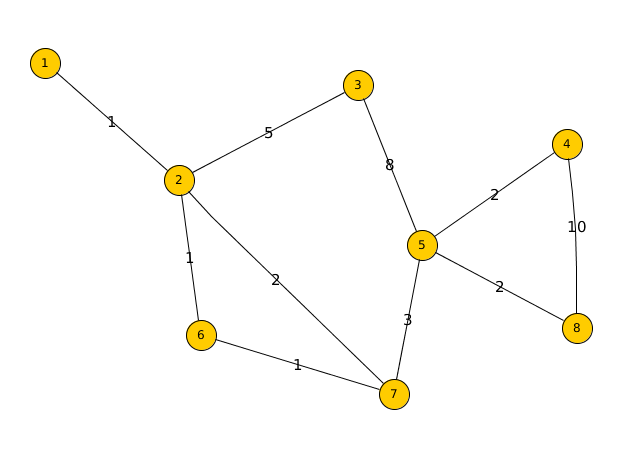
\includegraphics[scale=1]{imagenes/ej2.png}
		\caption{Instancia 1}
		\end{figure}
		
\begin{minipage}[t]{0.4\textwidth}
\begin{Verbatim}[frame=single,framesep=1cm,label= Ejemplo de entrada: instancia 1]
8 10 3
1 2 1
2 6 1
2 3 5
2 7 2
6 7 1
7 5 3
3 5 8
5 4 2
5 8 2
4 8 10
\end{Verbatim}
\end{minipage}
\hfill
\begin{minipage}[t]{0.4\textwidth}
\begin{Verbatim}[frame=single,framesep=1cm,label= Ejemplo de salida: instancia 1]
1 1 2 3 1 3 1 2
\end{Verbatim}
\end{minipage}
		
		En el ejemplo, primero el algoritmo ordena los nodos del grafo $G$ según el peso de sus máximas
		aristas. Es decir con el orden: 1 6 7 2 3 5 4 8 (en caso de empate, ordena según la suma de las aristas
		incidentes a los nodos). Luego, recorre esta lista de nodos y los va agregando de a uno al conjunto que
		dicho nodo agrega menos peso. Por ejemplo, primero agrega los nodos 1 y 6 al conjunto 1, y luego como el
		nodo 7 agrega 2 unidades de peso al conjunto 1 pero 0 al 2 (porque el conjunto 2 todavía no tiene ningún
		nodo), entonces agregamos el nodo 7 al conjunto 2. Con un razonamiento similar, en el próximo paso asignamos
		el nodo 2 al conjunto 3. De esta forma, se llega a la asignación de conjuntos 1 1 2 3 1 3 1 2 a cada uno de
		los nodos del grafo.
		
		\item Calcular el orden de complejidad de peor caso del algoritmo:
		El algoritmo que desarrollamos utiliza dos $for$, que van uno entre $1 \dots n$ y otro entre $1..k$.
		Si la complejidad de lo que hay adentro de estos ciclos es $O(T(n))$, entonces la complejidad total
		del algoritmo sería $O(knT(n))$. \\
		Dentro de estos ciclos lo que hacemos es determinar a qué conjunto $m$ agregar el nodo $i$. Para esto,
		lo que hacemos es recorrer para el nodo actual los $k$ conjuntos ($O(k)$) y en cada pasada calculamos 
		cuál sería el costo que generaría agregar el nodo $i$ al conjunto $k$. Esto lo hacemos de forma lineal 
		en $|V(G)|$, a partir de haber guardado el grafo $G$ en una estructura conveniente. Luego, 
		$T(n) = O(kn)$. \\
		Entonces, la complejidad de nuestro algoritmo en el peor caso es $ O(knT(n)) = O(k^2 n^2)$.
		
		\item Describir instancias de $k$-PMP para las cuales la heurística no proporciona una solución
		óptima. Indicar qué tan mala puede ser la solución respecto de la solución óptima.
		
		Veamos dos ejemplos en los que nuestra heurística no funciona correctamente. En estos ejemplos,
		la solución es infinitamente peor que la óptima.
		
		\begin{figure}[H]
			\begin{minipage}{.6\textwidth}
			\centering
			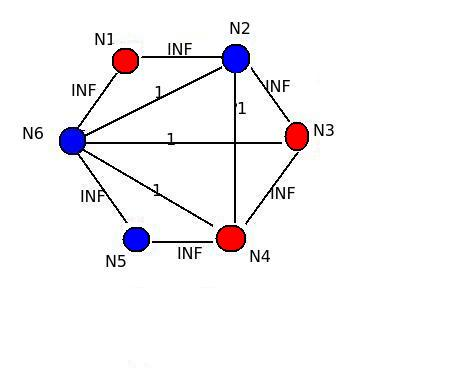
\includegraphics[width=.8\linewidth]{imagenes/ej3_11}
			\caption{Ejemplo 1 - solución de la heurística}
			\end{minipage}
			\begin{minipage}{.6\textwidth}
			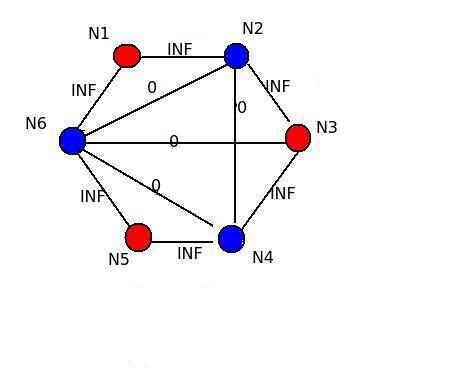
\includegraphics[width=.8\linewidth]{imagenes/ej3_12}
			\caption{Ejemplo 1 - solución óptima}
			\end{minipage}
		\end{figure}
		
		En el ejemplo 1, se busca una 2-PMP de un grafo $G$. Como las aristas internas tienen todas peso
		infinito, la solución óptima es la de la Figura 0.0.3, con peso 0. Sin embargo, la solución de 
		nuestra heurística devuelve la solución de la Figura 0.0.2, de peso infinito. El problema radica en 
		que cada par de nodos que son adyacentes, al sólo enfocarnos en agregarlo al conjunto que agrega el mínimo
		peso posible, terminamos agregando cada par de nodos del ciclo a conjuntos diferentes. El problema es que 
		al hacer esto nos quedamos sin conjuntos libres, y cuando tengamos que agregar el último nodo a algún
		conjunto, no va a importar cuál elijamos, en todos este va a agregar peso infinito. Este problema se
		generaliza para las $k$-PMP, siempre que suceda que al momento de procesar un nodo con todas sus aristas de
		peso infinito (o muy grande), todas estas aristas estén unidas a nodos que ya tienen asignados la totalidad
		de los $k$ conjuntos. Entonces, nos quedamos sin conjuntos para meter al nuevo nodo, y a cualquier conjunto de
		los ya creados que agreguemos este nodo, va a sumar un peso infinito (o muy grande).
		
		\begin{figure}[H]
		\begin{minipage}{.6\textwidth}
		\centering
		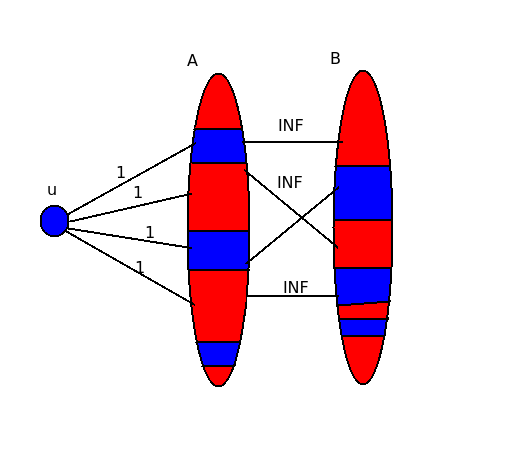
\includegraphics[width=.8\linewidth]{imagenes/ej3_21}
		\caption{Ejemplo 2 - solución de la heurística}
		\end{minipage}
		\begin{minipage}{.6\textwidth}
		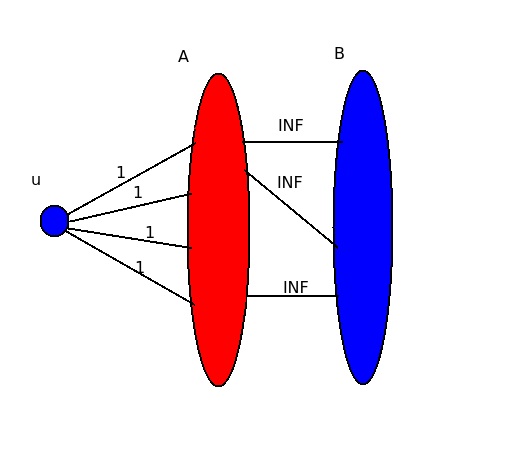
\includegraphics[width=.8\linewidth]{imagenes/ej3_22}
		\caption{Ejemplo 2 - solución óptima}
		\end{minipage}
		\end{figure}
		
		En el ejemplo 2, se busca la 2-PMP del grafo $G$. Dicho grafo es bipartito, a excepción del nodo extra que 
		agregamos, que está unido a un nodo en cada uno de los conjuntos. Si llamamos $V_{1}$ y $V_{2}$ a los
		conjuntos del subgrafo bipartito, asumimos que cada arista que va de un conjunto a otro pesa 1. Entonces, 
		la solución óptima sería la de la figura 0.0.6. Sin embargo, la solución de nuestra huerística podría ser la 
		dada por la figura 0.0.5. En un caso, el costo total es infinito y en el otro es $M$, con $M < \infty$. 
		Esto sucede porque al recorrer los nodos según los que tienen la mínima arista, primero se llenan los dos 
		conjuntos con nodos de $V_{1}$ y $V_{2}$ y por último se agrega el nodo extra. En este caso, si la heurística
		hubiera sido ordenar los nodos según la máxima arista, la solución hubiera sido la correcta. \\
		
		
		\item Realizar una experimentación que permita observar la performance del algoritmo en términos
		de tiempo de ejecución en función del tamaño de la entrada.
    \end{enumerate}
    
    \item Diseñar una heurística de búsqueda local para $k$-PMP y desarrollar los siguientes puntos:
    \begin{enumerate}
		\item Explicar detalladamente el algoritmo implementado. Plantear al menos dos vecindades disintas
		para la búsqueda. \\
		En el algoritmo que implementamos seguimos los siguientes pasos:
		\begin{enumerate}
			\item asignamos de forma aleatoria uno de los $k$ conjuntos a cada nodo
			\item mientras haya alguna solución vecina mejor que la actual, actualizamos todos los
			      conjuntos de nodos y el peso de la solución
			\item repetimos los dos pasos anteriores hasta que no haya una solución vecina mejor ó, hasta
			      haberlo repetido una cantidad límite de $x$ veces.
		\end{enumerate}
		La razón por la cual repetimos el proceso para varias soluciones iniciales es porque dependiendo
		de la solución inicial que consideremos, hallaremos un mínimo local distinto. Con lo cuál, para
		que la probabilidad de hallar el mínimo global sea lo más alta posible, hay que considerar 
		la mayor cantidad de soluciones iniciales distintas posible.
		
		Las dos vecindades que definimos fueron:
		\begin{enumerate}
			\item para cada nodo, chequear si cambiándolo a algún otro conjunto, se podría reducir el costo
			      total de la solución. Un pseudocódigo para el algoritmo implementado sería:
			      
			      \begin{algorithm}
					\SetKwInOut{Input}{input}
					\SetKwInOut{Output}{output}
					  \Input{grafo $G$, solución parcial $v$}
					  \Output{modifica $v$ y genera una nueva solución parcial, $v'$}
					  
					  \For{cada nodo $i = 1 \dots n$}{
						\For{$j = $ cada conjunto $1 \dots k$}{
							costoDelNodoViejo = calcularCosto($G$, $v$, $i$) \\
							$v' = $ cambiar nodo $i$ al conjunto $j$ \\
							costoDelNodoViejo = calcularCosto($G$, $v'$, $i$) \\
							\If{costoDelNodoNuevo $<$ costoDelNodoViejo}{
								$v = v'$ \\
								actualizo costo de $v$ (en $O(1)$) \\
								res = 1 \\
							}
							\If{costoDelNodoNuevo $\geq$ costoDelNodoViejo}{
								res = 0 \\
							}
						}
					  }
					  return res \\
					\caption{Algoritmo de búsqueda local con vecindad 1}
					\end{algorithm}
			     \textbf{Nota: } La función calcularCosto(G,v,i) recorre los nodos adyacentes al nodo $i$, y acumula la suma
					            de las aristas que unen a $i$ con algún otro nodo adyacente a $i$ en la solución actual
			     
			\item para cada nodo, chequear si swappeandolo de conjunto con otro nodo ó mandándolo a un conjunto que esté
			      vacío se reduce el costo.
				  
				  \begin{algorithm}
					\SetKwInOut{Input}{input}
					\SetKwInOut{Output}{output}
					  \Input{grafo $G$, solución parcial $v$}
					  \Output{modifica $v$ y genera una nueva solución parcial, $v'$}
					  
					  \For{ cada nodo $i = 1 \dots n$ }{
						
						nodoModificado1 = -1 \\
						nodoModificado2 = -1 \\
						costoOriginal = v.second \\
						
						\For{ cada nodo $j = 1 \dots n$ }{
						
							costoNodoViejo1 = calcularCosto(G,n,v,i) \\
							costoNodoViejo2 = calcularCosto(G,n,v,j) \\
							
							swap(v.first[i], v.first[j])	// swapeo los nodos de conjunto \\
							
							costoNodoNuevo1 = calcularCosto(G,n,v,i) \\
							costoNodoNuevo2 = calcularCosto(G,n,v,j) \\
							
							costoViejo = costoNodoViejo1 + costoNodoViejo2 \\
							costoNuevo = costoNodoNuevo1 + costoNodoNuevo2 \\
							
							\eIf{costoNuevo $<$ costoViejo}{
								res = 1 \\
								v.second = v.second - costoViejo + costoNuevo \\
								nodoModificado1 = i \\
								nodoModificado2 = j 		// guardo los nodos con los que hice el swap \\
							}{
								swap(v.first[i], v.first[j])	// reestablezco el swapeo que habíamos hecho \\
							}
							
							
						}
						
						conjuntoVacio = indice de algun conjunto vacio 	// O(k) \\
						\If{ conjuntoVacio es un indice valido }{
							encontreMejorSeparado = 0 \\
							meGuardoCosto = v.second \\
							meGuardoNodoCambiado = -1 \\
							
							\If{ hicimos algun swap }{
								swap(v.first[nodoModificado1], v.first[nodoModificado2]) // deshacemos el swap para ver si convenia cambiar
																							algun nodo al conjunto vacio\\
							}
							
							\For{ cada nodo $j = 1 \dots n$ }{
								deltaCostoDelCambio = calcularCosto(G,n,v,j) \\
								costoDelCambio = costoOriginal - deltaCostoDelCambio \\
								\If{costoDelCambio $<$ meGuardoCosto}{	// si encontre un nodo mejor que el ultimo encontrado \\
									meGuardoCosto = costoDelCambio \\
									meGuardoNodoCambiado = j \\
									encontreMejorSeparado = 1 // quiere decir que es mejor cambiar un nodo a un conjunto vacio que 
																 hacer el swap que habiamos hecho\\
								}
							}
							
							// Ahora me fijo si debo reestablecer el swapeo que habia hecho o no \\
							\eIf{encontreMejorSeparado == 1 y habiamos hecho algun swap}{
								swap(v.first[nodoModificado1], v.first[nodoModificado2]) \\
							}{
								v.second = meGuardoCosto \\
								v.first[meGuardoNodoCambiado] = conjuntoVacio \\
								Actualizo la cantidad de nodos que tengo por conjunto 	// O(1) \\
								
							}				
						}
					}
					  
					\caption{Algoritmo de búsqueda local con vecindad 2}
					\end{algorithm}
				  
		\end{enumerate}
		
		En el caso de la primera  y segunda vecindad, una instancia posible y su solución serían (partiendo de la solución 
		aleatoria inicial 3 3 3 3 1 2 3 3). \\

		
\begin{minipage}[t]{0.4\textwidth}
\begin{Verbatim}[frame=single,framesep=1cm,label= Ejemplo de entrada]
8 10 3
1 2 1
2 6 1
2 3 5
2 7 2
6 7 1
7 5 3
3 5 8
5 4 2
5 8 2
4 8 10
\end{Verbatim}
\end{minipage}
\hfill
\begin{minipage}[t]{0.4\textwidth}
\begin{Verbatim}[frame=single,framesep=1cm,label= Ejemplo de salida: vecindad 1]
2 1 3 2 1 2 3 3
\end{Verbatim}
\hfill
\begin{Verbatim}[frame=single,framesep=1cm,label= Ejemplo de salida: vecindad 2]
3 3 3 3 1 3 3 2
\end{Verbatim}
\end{minipage}
		
		Vale aclarar que es esperable que, para distintas vecindades, en general nos den resulados diferentes. Además, en este ejemplo
		en particular, usando la vecindad 2 obtenemos una solución muy mala (de costo total igual a 10), mientras que para la vecindad 1,
		obtenemos una solución buena (costo total igual a 0). En este ejemplo en particular, como inicialmente no hay ningún conjunto vacío,
		cuando utilizemos la vecindad 2, sólo se van a efectuar swaps de nodos entre conjuntos, y la cantidad de nodos que hay en cada conjunto
		se va a mantener invariante (si hubiera algún conjunto vacío de seguro se le agregaría un nodo a dicho conjunto, ya que al cambiar un nodo
		a un conjunto vacío, se reduce mucho la porción del costo total asociada a dicho nodo). \\
		
		\item Calcular el orden de complejidad temporal de peor caso de una iteración del algoritmo de búsqueda local
			  (para las vecindades planteadas). Y si es posible, dar una cota superior para la cantidad de iteraciones
			  de la heurística. 
			  
			  En el caso de la vecindad 1, el costo de cada iteración del algoritmo de búsqueda local es $O(kn^2)$ y esto
			  se deduce fácilmente del pseudocódigo presentado en el punto anterior (empleamos dos $for$, y adentro de uno
			  de estos, llamamos a una función que calcula el costo de agregar el nodo a un conjunto, cuyo costo computacional
			  es $O(n)$, pues cada nodo es adyacente como máximo a $n-1$ nodos).
			  
			  En el caso de la vecindad 2, el costo de cada iteración del algoritmo e búsqueda es $ O(n^3) $. Esto se deduce
			  del pseudocódigo presentado más arriba: el algoritmos consta de una serie de ciclos $for$, dentro de los
			  cuáles se llama a la función $calcualrCosto$, que tiene complejidad temporal $O(n)$. Observando el pseudocódigo,
			  se llega a que la complejidad es $T(n) = O(n^3) + O(nk) + O(n^3) = O(n^3) $.
			  
	    \item Realizar una experimentación que permita observar la performance del algoritmo comparando los tiempos
			  de ejecución y la calidad de las soluciones obtenidas, en función de las vecindades utilizadas y elegir,
			  si es posible, la configuración que mejores resultados provea pra el grupo de instancias utilizado.
    \end{enumerate}
\end{enumerate}





%% =====================================================================

\end{document}
